\section{Physics motivation\label{sec:physHI}}
\label{sec:physics}

{\bf [Yen-Jie working on this section]}

In this Section we discuss the physics performance of the upgraded L1 trigger system for the 2018 high luminosity PbPb run
using three examples of measurements using rare probes. 
The performance of the upgraded system, which uses background subtraction for L1 event rejection and provides 
access to the full expected luminosity of 3~nb$^{-1}$ is compared to that of the current system. 
These examples illustrate the large improvements in statistical precision afforded by the  improved 
ability to select jet events and high \pt\ particles during high luminosity PbPb collisions. 


%Studies of high \pt\ jet and charged particle production in the 2010 and 2011 PbPb data sets have helped to elucidate the nature of parton energy loss in hot nuclear matter. Parton energy loss was characterized using a wide range 
%of different signatures, ranging from the the dijet energy imbalance in central collisions and the suppression of single particle
%spectra at the highest \pt\ to modifications of jet shapes and fragmentation patterns~\cite{Chatrchyan:2011sx,Aamodt:2010jd,Alice:dihadron,CMS:2012aa,Chatrchyan:2012nia,Aad:2010bu,atlas:2012is,Chatrchyan:2012gt,Chatrchyan:2012gw}. 

Below we discuss a selection of measurements which exploit the future high luminosity data sets to 
provide important insights into the parton energy loss mechanism and heavy flavor particle production:

\begin{enumerate}
\item The flavor dependence of jet quenching is a crucial important test ground for various parton energy loss models. 
Compared to light quarks, heavy quarks are expected to suffer from smaller radiative energy loss when passing 
through the medium because gluon radiation is suppressed at angles smaller than the ratio of the quark mass $M$ to 
its energy $E$~\cite{Dokshitzer:2001zm}. This effect (and its disappearance at high \pt) can be studied using tagging
of b-decays and b-jets.
\item Compared to quarks, gluons are expected to suffer a larger 
energy loss because of the larger color factors. This effect can be studied using three-jet events.
\item Measurements of the single particle azimuthal anisotropy at very high \pt\ give access to the in-medium path-length 
dependence of energy loss. The azimuthal anisotropy as a function of charged particle \pt\ also yields 
important information about the parton energy dependence of the energy loss.
\end{enumerate}

These and other measurements rely on a sufficiently selective jet and heavy flavor meson trigger to provide access to the 
full delivered luminosity and a large minimum-bias sample.  Data collected during the 2015 PbPb run were used to estimate physics reach  
for a future high-luminosity run (assuming $L_{int} =$3~nb$^{-1}$) for these three physics cases. 
%Using typical thresholds of leading jet \pt\ $>100$~GeV/c, Figure~\ref{fig:efficiency_comparison} shows that 
%with the upgraded system (labeled ``Stage-1 system'' in the plots) sufficient rejection factors can be 
%achieved to sample the full delivered luminosity. For the current system (labeled ``Current system'' in the 
%plots), the rejection factor at L1 is limited to about two, requiring a large prescale factor to be applied
%due to bandwidth constraints in the detector front end readout. Figure~\ref{fig:aj_2015} to 
%\ref{fig:xT_scaling} show the effect of the resulting difference in statistical reach 
%for the physics examples discussed below.

\begin{figure}[!ht]
\begin{center}
%\includegraphics[width=.60\textwidth]{fig/heavyIon//efficiency_comparison_l1primitives.pdf}
\caption{The jet finder is applied to minimum bias data from 2011 without
event selection using the L1 primitives present in the RAW data. The
fraction of events which have a jet above a given $E_t$ threshold is plotted
as a function of that threshold. Note that the threshold is applied to the
L1 jet energy and does not correspond to the HLT or offline jet energy
scales.}
\label{fig:efficiency_comparison}
\end{center}
\end{figure}


\subsection{Nuclear Modification Factors of Heavy Flavor Mesons}
{\bf [To be updated]}

A proof of principle measurement of b-jet production in PbPb collisions has
been performed with the 2011 data.  
This measurement of the b-jet to inclusive jet ratio, however, suffers from
large statistical and consequently also systematic uncertainties.  
The golden measurement in the b-jet channel would be a measurement of the
dijet asymmetry for doubly-tagged b-jets, 
where we expect systematic uncertainties to be small, and to mostly cancel
with respect to the corresponding light-quark jet measurements.  
The rate of doubly-tagged b-jets has been estimated based on the number
of inclusive dijets in the 2011 sample.  
The b-jet to inclusive jet ratio was measured to be approximately 0.03 in pp
collisions at 7 TeV, as well as in 2.76 TeV PbPb collisions, with 
significantly larger uncertainties in the latter case.  Of these b-jets only
about 20\% will be produced back-to-back with another b-jet, 
in the so-called flavor creation mode.  Using a simple secondary vertex
tagger, one can achieve about 50\% tagging efficiency in PbPb.  
For doubly-tagged jets, then, one only obtains a tagging efficiency of 25\%,
but with a purity close to unity.  
Assuming $x_{T}$ scaling with an exponent of $n = 4.5$, the yield of jets at
fixed \pt\ increases by a factor of 5 for the increased collision energy 
expected in 2015.  

The distribution of the dijet asymmetry variable $A_{J}$ is defined as the
difference between the leading and subleading jet transverse momenta,
divided by their sum.  
The $A_{J}$ distribution for doubly tagged b-jets is estimated from the
inclusive jet $A_{J}$ distribution, 
scaling the uncertainties to those expected from $1.5\ {\rm nb^{-1}}$ of data at
5.5 TeV, with a tagging efficiency of 25\%.  This distribution is shown in
Figure~\ref{fig:aj_2015} for the 10\% most central PbPb events.  
The kinematic cuts on the leading and sub-leading jets are \pt $>$ 100 GeV/c
and \pt $>$ 30 GeV/c, respectively, for jets in $|\eta| < $2.  


\begin{figure}[!ht]
\begin{center}
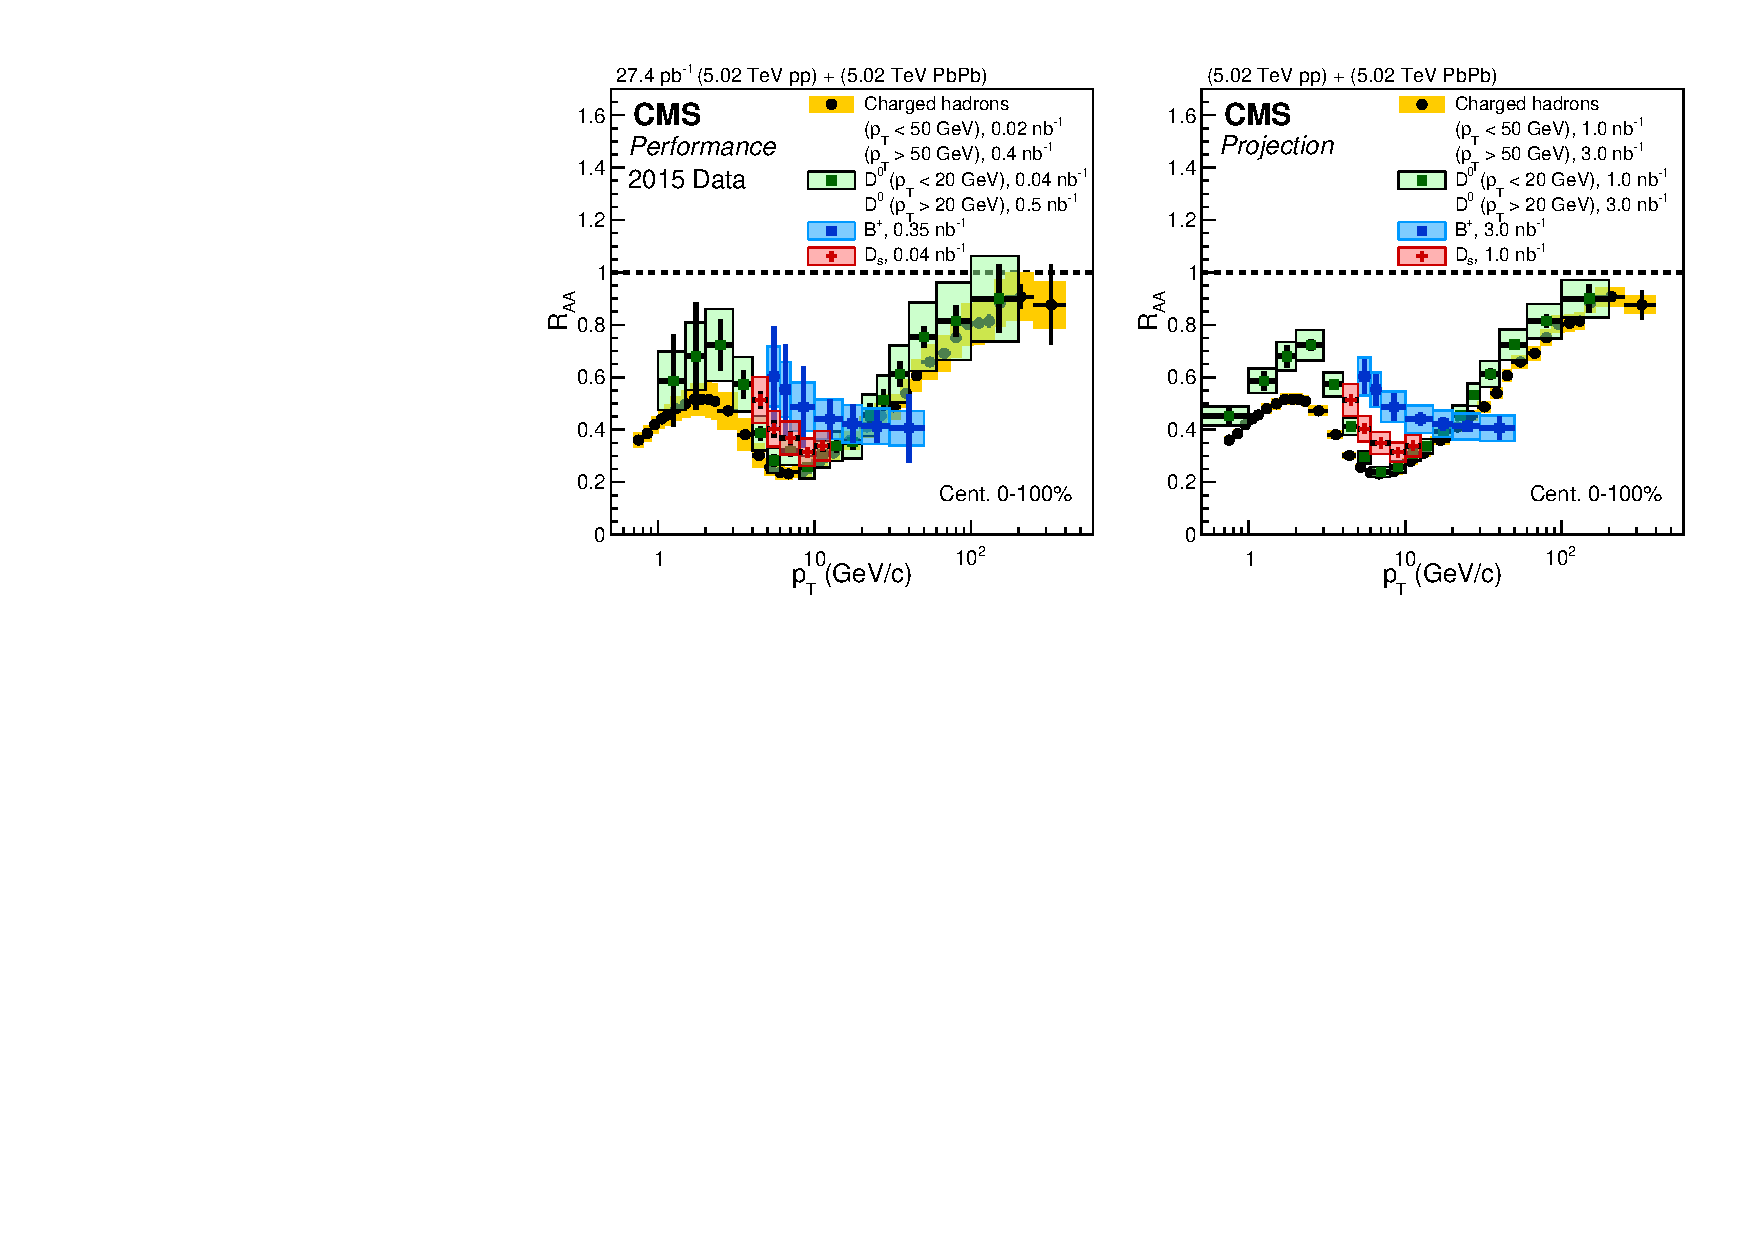
\includegraphics[width=.90\textwidth]{figures/cRAA_lumiTG_3_lumiMB_1_v2.pdf}
\caption{Nuclear modification factors of charged particles, $D^0$, $D_s$ and $B^+$ mesons with 2015 data (left panel) and the statistics expected with L1 trigger rate upgrade.}
\label{fig:aj_2015}
\end{center}
\end{figure}

\subsection{Ellipic Flow of Heavy Flavor Mesons}

Events with three or more jets in the final state originate from hard gluon radiation and 
other higher-order QCD processes. A measurement of the inclusive 3-jet to 2-jet cross section 
ratio ($R_{32}$) is an interesting testing ground of pQCD, with possible modification of 
parton shower and gluon jet-quenching in QGP, because major systematic uncertainties such as 
jet energy scale, reconstruction efficiency and integrated luminosity measurement largely cancel. 
The expected number of 3-jet events at 5.5 TeV is estimated based on the observed statistics in the 2011 data sample, 
in which we recorded about 106 3-jet events and 8225 dijet events, with all jets having \pt\ $>$ 100 \GeVc.  
The ratio from PYTHIA events, with uncertainties scaled to the expected
2015 statistics, is shown in Figure~\ref{fig:r32_2015}. 
With the upgrade L1 system, $R_{32}$ measurements as a function of the
average \pt\ of the two leading jets are made possible.


\subsection{$D^0$-Jet and $D^0$-hadron correlations}

The expected \pt\ reach of charged particle spectra is presented in
Figure~\ref{fig:xT_scaling}.
With the upgraded L1 system and improved L1 jet trigger with underlying
event subtraction,
a large improvement in correlation between the track \pt\ and L1 jet \pt\ can be
achieved, as shown in
Figure~\ref{fig:trigEff_track2015_central} (left) for 0--30\% centrality and
Figure~\ref{fig:trigEff_track2015_peripheral} (left) for 40--100\%
centrality.
Therefore, it is feasible to use high \pt\ L1 jet as a seed to the high \pt
track high-level trigger.
In this way, one can fully access the total delivered luminosity to
significantly extend the track \pt\ reach in the high luminosity PbPb run 
(red markers in Figure~\ref{fig:xT_scaling}),
which is crucial for studying the high \pt\ charged particle suppression and
anisotropic azimuthal distribution.
As shown on the right hand sides of
Figure~\ref{fig:trigEff_track2015_central} and
\ref{fig:trigEff_track2015_peripheral},
by selecting L1 jet \pt\ of 40--50 GeV/c, one can maintain 100\%
efficiency for the high \pt\ track trigger
in both central (\pt\ $>$ 60 GeV/c) and peripheral (\pt\ $>$ 40 GeV/c) heavy ion collisions, 
while the L1 jet rate can be well controlled. Unprescaled access to high \pt\ 
single particle production provides the basis for a large number of 
important energy loss analyses complementary to jet-trigger bases approaches.


\begin{figure}[!ht]
\begin{center}
%\includegraphics[width=.60\textwidth]{fig/heavyIon//r32_2015.pdf}
\caption{The ratio of 3-jet to 2-jet events ($R_{32}$ )as a function of the
average \pt\ of the two leading jets for \pt\ $> $ 100 GeV/c 
in the ten percent most central collisions expected in the 2015 PbPb Run.}
\label{fig:r32_2015}
\end{center}
\end{figure}

\begin{figure}[!ht]
\begin{center}
%\includegraphics[width=.50\textwidth]{fig/heavyIon//HighPtTrackReach_xTscaling_20121216.pdf}
\caption{Track \pt\ distribution for 2.76 TeV PbPb in 2011 with a total
integrated luminosity
         of 150$\mu$b$^{-1}$ (solid black), projection to 5.5 TeV in 2015
based on $x_T$ scaling 
         without upgraded L1 trigger (open red), and with upgraded L1
trigger (solid red).}
\label{fig:xT_scaling}
\end{center}
\end{figure}

\begin{figure}[!ht]
\begin{center}
%\includegraphics[width=.48\textwidth]{fig/heavyIon//JetvsTrack_PU1_centmin0_centmax12_20130214.pdf}
%\includegraphics[width=.48\textwidth]{fig/heavyIon/efficiency_trackpt_PU1_centmin0_centmax12_20130214.pdf}
\caption{Leading L1 jet $E_T$, with upgraded L1 system, vs leading track
\pt\ in 0-30\% PbPb collisions
at 2.76 TeV (left), and efficiency turn-on curve as a function of leading
track \pt\ for L1 jet $E_T$
thresholds of 40, 50 and 60 GeV (right).}
\label{fig:trigEff_track2015_central}
\end{center}
\end{figure}

\begin{figure}[!ht]
\begin{center}
%\includegraphics[width=.48\textwidth]{fig/heavyIon//JetvsTrack_PU1_centmin16_centmax40_20130214.pdf}
%\includegraphics[width=.48\textwidth]{fig/heavyIon//efficiency_trackpt_PU1_centmin16_centmax40_20130214.pdf}
\caption{Leading L1 jet $E_T$, with upgraded L1 system, vs leading track
\pt\ in 40-100\% PbPb collisions
at 2.76 TeV (left), and efficiency turn-on curve as a function of leading
track \pt\ for L1 jet $E_T$
thresholds of 40, 50 and 60 GeV (right).}
\label{fig:trigEff_track2015_peripheral}
\end{center}
\end{figure}
